\mysection{Vizualizované algoritmy}

\begin{itemize}

    \item broadcast -- \textit{ako povedať novú klebetu všetkým v sieti?}
    \item voľba šéfa na úplnom grafe -- \textit{ako sa spomedzi niekoľkých identických programov
    dá zvoliť jeden šéf? a čo ak pri tom chceme poslať čo najmenej správ?}
    \item traverzovanie -- \textit{ako prehľadať celý graf podávaním si jediného tokenu?}
\end{itemize}

\begin{figure}
\vspace{-1cm}
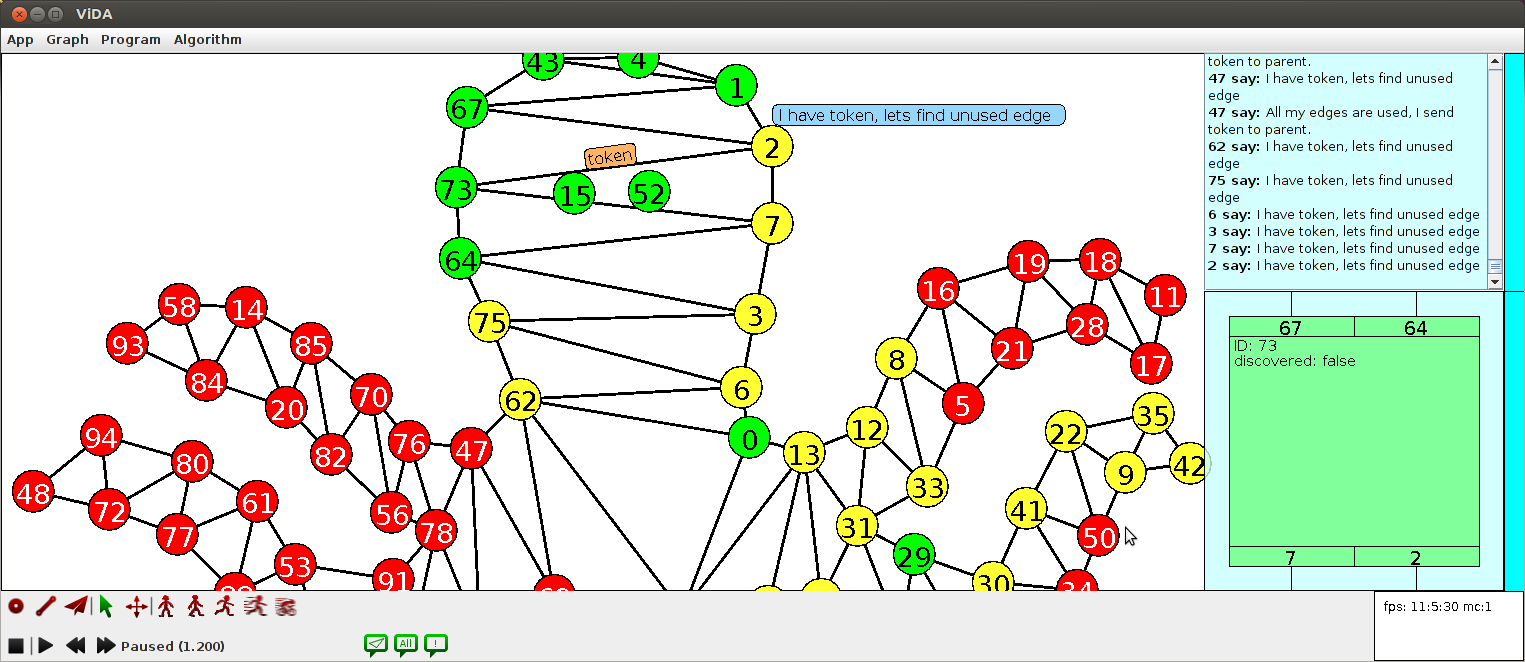
\includegraphics[width=\columnwidth]{traverz}
\vspace{-1cm}
\caption{Traverzovanie -- zelené vrcholy sú nenavštívené, oranžové sú navštívené, červené sú úplne
vybavené, teda už preskúmali všetkých susedov}
\vspace{-1cm}
\end{figure}
    
\mysection{Nástroje}

\begin{itemize}
    \item úprava grafu
    \begin{itemize}
        \item pridávanie, mazanie, editovanie, hýbanie vrcholov a hrán
        \item ukladanie, automatické generovanie rôznych typov a veľkostí
        \item verifikácia -- napr. niektoré algoritmy sú určené len pre úplné grafy
    \end{itemize}
    \item časovanie správ
    \begin{itemize}
        \item možnosť chytiť správu a presunúť ju na iné miesto na hrane
        \item nastavovanie rýchlostí hrán a správ
    \end{itemize}
    \item selekcia -- zobrazovanie dodatočných informácií
\end{itemize}
\vspace{-0.5cm}

\mysection{Spôsob vizualizácie}

\begin{itemize}
    \item zobrazovanie udalostí priamo v grafe -- netreba vrtieť hlavou a hľadať, čo sa kde deje,
    informácie sa zobrazujú tam, kde sa ich to týka, všetko pomocou \emph{vyskakovacích bubliniek}
    \item interaktivita -- \emph{čo by sa stalo, keby\dots?} užívateľ môže priamo ovplyvňovať, čo sa
    stane
    \item detekcia a vysvetlenie zaujímavých udalostí -- keď sa niečo stane, aplikácia sa pozastaví
    a vysvetlí 
    \emph{čo sa stalo, prečo sa to stalo, kde sa to stalo a čo sa bude diať ďalej.}
\end{itemize}

\begin{figure}
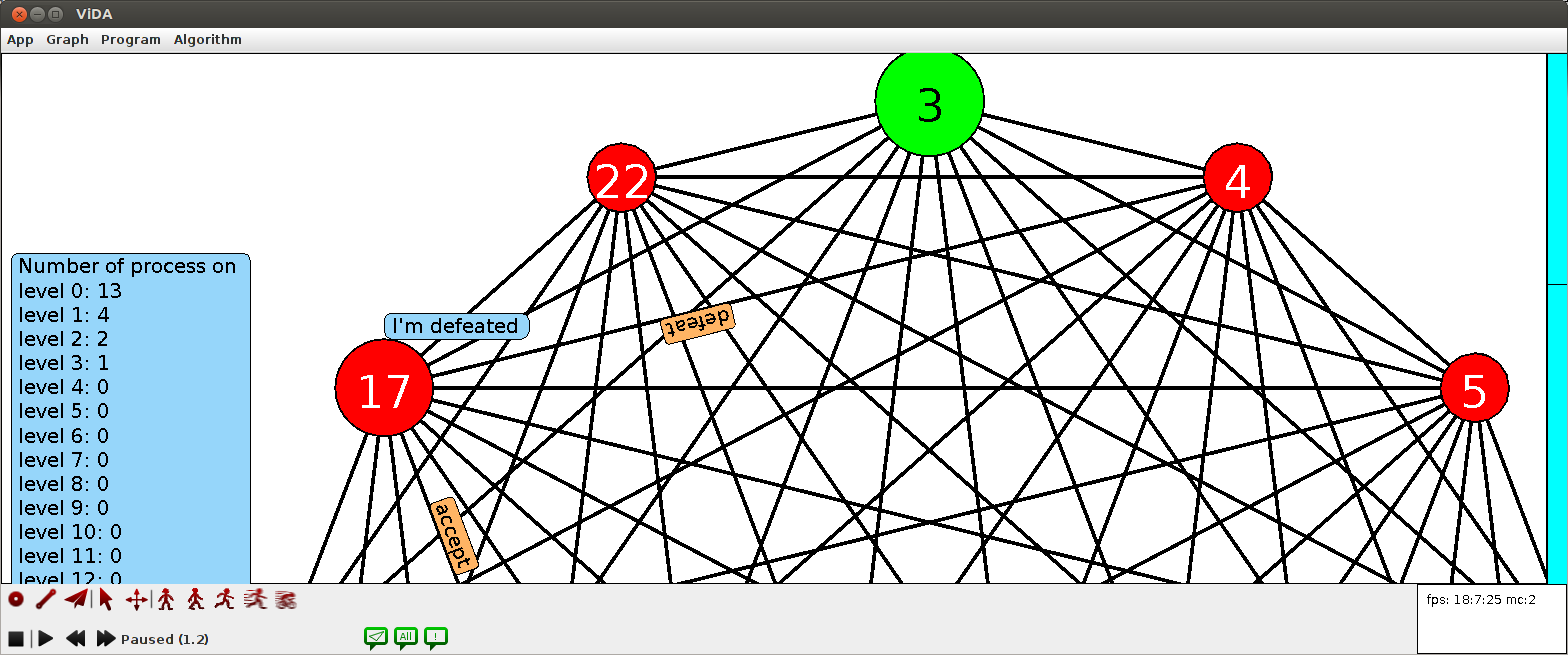
\includegraphics[width=\columnwidth]{le}
\vspace{-1cm}
\caption{Informácie priamo v grafe -- intuitívne spojenie vizuálnych a hodnotových
vlastností, napr. veľkosť vrcholu = level, farba vrcholu = stav (napr. červený =
mŕtvy/porazený/neaktívny). Algoritmus na voľbu šéfa}
\end{figure}


\begin{figure}
\vspace{-1cm}
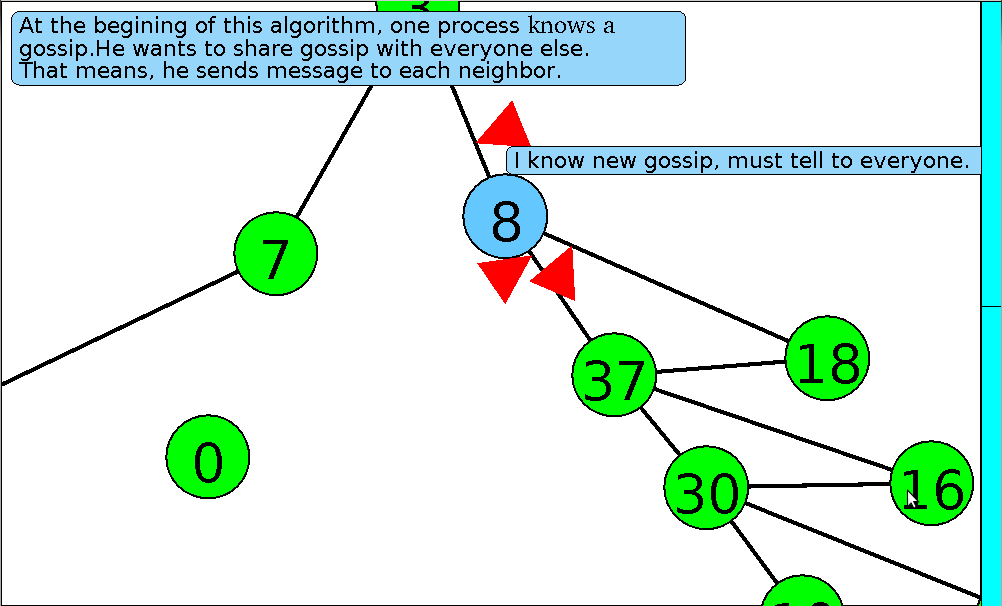
\includegraphics[width=\columnwidth]{bfs}
\vspace{-1cm}
\caption{Zobrazovanie informácií v bublinkách. Algoritmus broadcast.}
\vspace{-1cm}
\end{figure}

\mysection{Vlastné vizualizácie}

\begin{itemize}
    \item možnosť vytvárania vlastných vizualizácií
    \item knižnica vidalib
        \begin{itemize}
            \item jednoduchá knižnica v C++ komunikujúca s naším programom
            \item poskytnutie celej palety nástrojov -- vyskakovacie bublinky, zmena farby a
            veľkosti vrcholov \dots
        \end{itemize}
    \item hlbšie pochopenie algoritmu po jeho naimplementovaní
    \item potešenie z vlastných fungujúcich algoritmov
\end{itemize}

%TODO popis konkretnych algoritmov

\mysection{Plány do budúcnosti}


\begin{itemize}
    \item ďalšie algoritmy
    \begin{itemize}
        \item GHS -- \emph{voľba šéfa na všeobecnom grafe}
        \item KKM -- \emph{voľba šéfa s využitím traverzovania}
        \item routing -- \emph{smerovanie dát v sieti. Kam poslať paket, aby sa dostal do cieľa?}
        \item problém dohody
    \end{itemize}
    \item nové nástroje na prácu s grafom, správami, ďalšie nástroje na vizualizáciu
    \item viac zábavy, viac interaktivity -- \emph{užívateľ sa môže zahrať na \clqq zá\-ke\-rá\-ka\crqq\ a snažiť sa
    donútiť algoritmus, aby poslal čo najviac správ}
    \item podpora viacerých programovacích jazykov
\end{itemize}

%TODO plany do buducnosti
